% 编译：xelatex lock_report.tex（运行两遍）
\documentclass[UTF8,a4paper,10pt,fontset=fandol]{ctexart}
\usepackage[margin=2cm]{geometry}
\usepackage{graphicx,booktabs,hyperref,xcolor}
\hypersetup{colorlinks=true,linkcolor=blue!50!black}
\setlength{\emergencystretch}{3em}
\newcommand{\code}[1]{\texttt{\detokenize{#1}}}
\begin{document}
\begin{center}
{\Large\bfseries 互斥同步与锁竞争优化实验报告}\\[0.5em]
姓名：赵心瑞\qquad 学号：24307140096
\end{center}

\section{实现方案}
原始物理内存分配器使用一条空闲页链表和一把全局锁，多 CPU 并发分配、释放时容易竞争。本实验在 \code{lock} 分支修改 \code{kernel/kalloc.c}，将其改为每 CPU 一条链表、一把自旋锁，并支持跨 CPU 偷取页面。

\begin{enumerate}
\item \textbf{数据结构与初始化：}将 \code{kmem} 改为大小为 \code{NCPU} 的数组，每个元素保存独立的锁和 \code{freelist}。\code{kinit()} 先初始化所有锁，再调用一次 \code{freerange()}。初始空闲页集中在执行初始化的 CPU 上。
\item \textbf{释放页面：}\code{kfree()} 保留地址检查和页面填充，通过 \code{cpuid()} 获取当前 CPU 编号，在对应锁保护下将页面插入本地链表头。
\item \textbf{分配与偷页：}\code{kalloc()} 优先从本地链表摘取页面。本地为空时，先释放本地锁，再依次检查其他 CPU 的链表，在目标锁保护下取走一页；遍历后仍未获得页面则返回 0。
\end{enumerate}

通过配对的 \code{push_off()/pop_off()} 关闭本 CPU 中断并恢复原状态，使获取和使用 CPU 编号期间不会因时钟抢占而迁移。所有链表读写均持有对应锁；偷页时一次只持有一把锁，避免多锁循环等待。分配后的 \code{memset()} 在锁外执行，缩短临界区。

\section{测试结果与分析}
在 QEMU 三 CPU 环境下运行测试。\code{#test-and-set} 表示获取锁失败后的重试次数；下表统计各 \code{kmem} 锁的累计竞争次数或增量，结果截图见图\ref{fig:kalloc}。
\begin{center}
\begin{tabular}{lrr}
\toprule
指标 & 原始实现 & 优化后\\
\midrule
test1 竞争次数 & 32926 & 0\\
test3 新增竞争次数 & 43531 & 7502\\
test2 空闲页数量 & 32465 & 32465\\
kalloctest 结果 & test1、test3 FAIL & test1--test3 全部 OK\\
\bottomrule
\end{tabular}
\end{center}
原版 test3 增量为 $76457-32926=43531$，优化后为 $7502-0=7502$，减少约 $82.8\%$。这次测试中，本地链表使常规操作避开全局锁竞争；跨 CPU 偷页仍需访问其他锁，因此竞争未完全消失。计数受运行时序影响，这里比较的是本次测试结果，而非运行时间加速比。

优化前后空闲页数量一致，test2 通过。\code{usertests sbrkmuch} 输出 \code{test sbrkmuch: OK}，\code{usertests -q} 最终输出 \code{ALL TESTS PASSED}（图\ref{fig:user}），表明本次实现通过大量内存申请及用户回归测试。回归截图中的部分用户态异常属于非法访问测试，其对应测试最终为 OK。

\clearpage
\section{测试截图}
\begin{figure}[htbp]
\centering
\begin{minipage}[t]{0.48\textwidth}
\centering
\textbf{优化前}\\[0.5em]
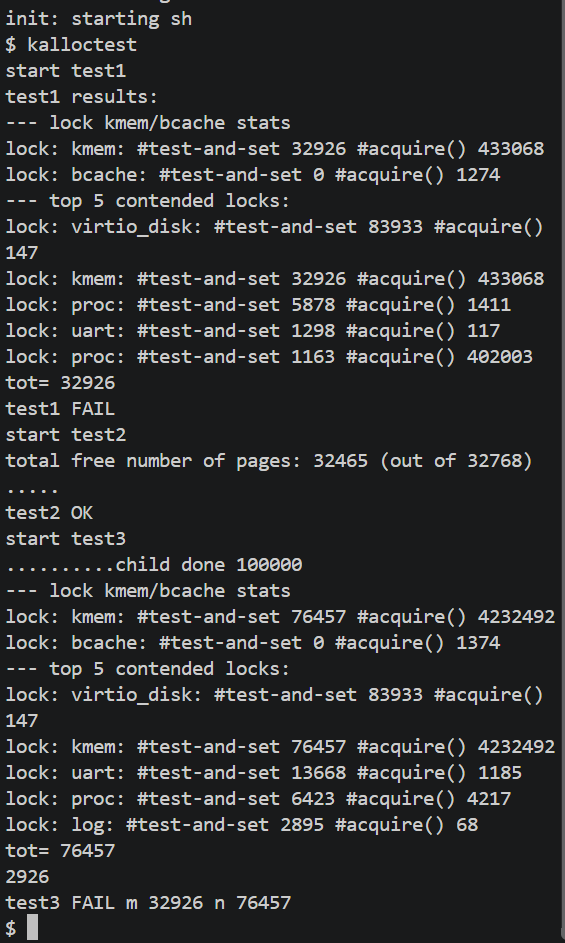
\includegraphics[width=\linewidth,height=0.78\textheight,keepaspectratio]{result-1.png}
\end{minipage}\hfill
\begin{minipage}[t]{0.48\textwidth}
\centering
\textbf{优化后}\\[0.5em]
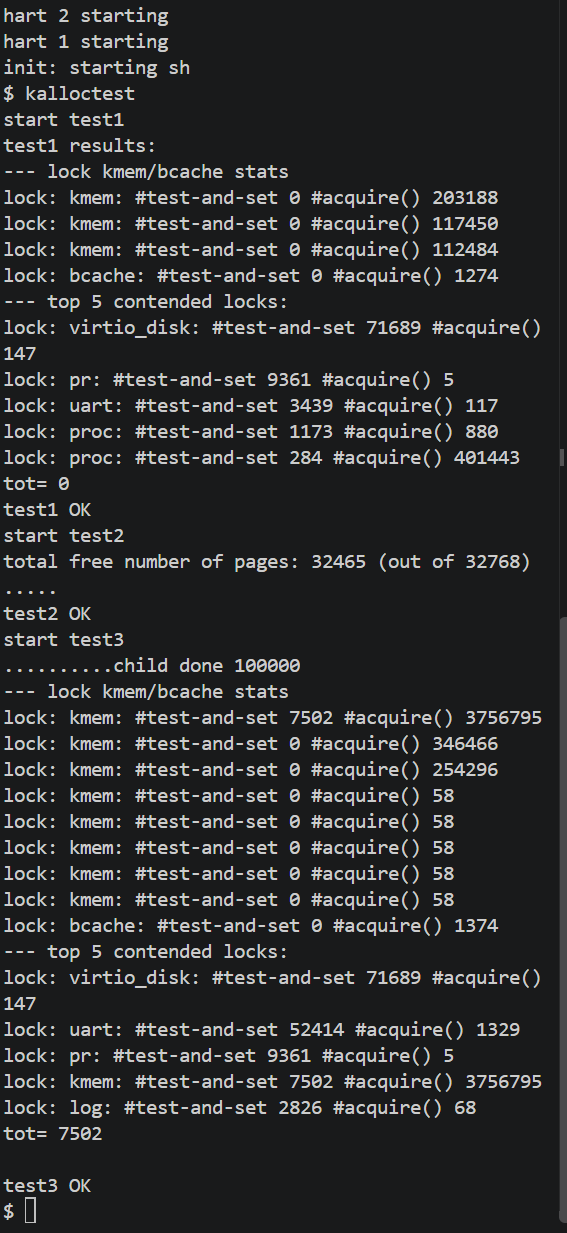
\includegraphics[width=\linewidth,height=0.78\textheight,keepaspectratio]{result-2.png}
\end{minipage}
\caption{kalloctest 优化前后对比。}\label{fig:kalloc}
\end{figure}

\clearpage
\begin{figure}[htbp]
\centering
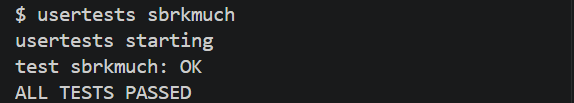
\includegraphics[width=0.85\textwidth]{result-3.png}\\[1.5em]
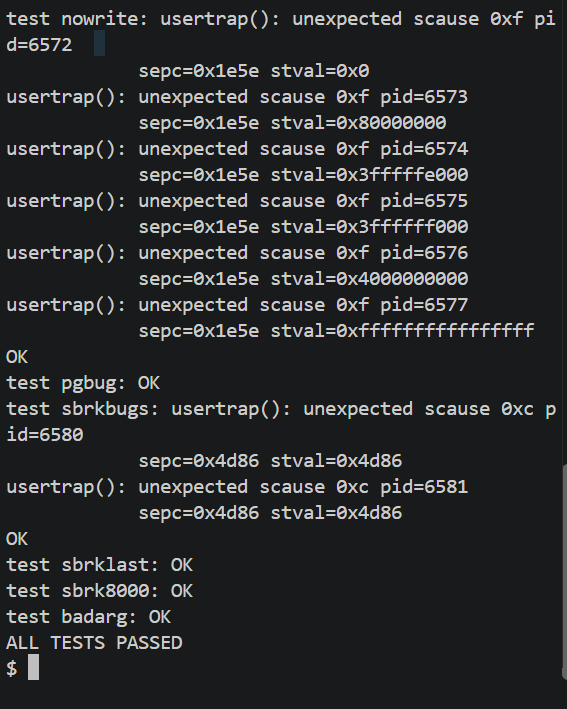
\includegraphics[width=0.78\textwidth,height=0.68\textheight,keepaspectratio]{result-4.png}
\caption{usertests sbrkmuch 通过，以及 usertests -q 最终全部通过。}\label{fig:user}
\end{figure}
\end{document}
